%%%%%%%%%%%%%%%%%%%%%%%%%%%%%%%%%%%%%%%%%
% Short Sectioned Assignment
% LaTeX Template
% Version 1.0 (5/5/12)
%
% This template has been downloaded from:
% http://www.LaTeXTemplates.com
%
% Original author:
% Frits Wenneker (http://www.howtotex.com)
%
% License:
% CC BY-NC-SA 3.0 (http://creativecommons.org/licenses/by-nc-sa/3.0/)
%
%%%%%%%%%%%%%%%%%%%%%%%%%%%%%%%%%%%%%%%%%

%----------------------------------------------------------------------------------------
%	PACKAGES AND OTHER DOCUMENT CONFIGURATIONS
%----------------------------------------------------------------------------------------

\documentclass[paper=a4, fontsize=11pt]{scrartcl} % A4 paper and 11pt font size

\usepackage[usenames,dvipsnames,x11names]{xcolor} % Colors

\usepackage[T1]{fontenc} % Use 8-bit encoding that has 256 glyphs
\usepackage{fourier} % Use the Adobe Utopia font for the document - comment this line to return to the LaTeX default
\usepackage[english]{babel} % English language/hyphenation
\usepackage{amsmath,amsfonts,amsthm} % Math packages

\usepackage{sectsty} % Allows customizing section commands
\allsectionsfont{\centering \normalfont\scshape} % Make all sections centered, the default font and small caps

\usepackage{tikz}
\usepackage{pgfplots}
\usetikzlibrary{plotmarks}

\usepackage{booktabs}  % for \toprule, \midrule, and \bottomrule macros 
\usepackage{longtable} % Tables spanning page boundaries
\usepackage{tabularx}  % for 'tabularx' environment and 'X' column type
\usepackage{ragged2e}  % for '\RaggedRight' macro (allows hyphenation)
\newcolumntype{Y}{>{\RaggedRight\arraybackslash}X} 
\usepackage{paralist} % Inline list environment
%\usepackage{tablefootnote}

\usepackage{acronym}
\usepackage[inline]{enumitem}
\usepackage{fancyhdr} % Custom headers and footers
\usepackage{graphicx} % Allow use of images
\usepackage{lastpage}
\usepackage{listings}
\usepackage{multirow}

\pagestyle{fancyplain} % Makes all pages in the document conform to the custom headers and footers
\fancyhead{} % No page header - if you want one, create it in the same way as the footers below
\fancyfoot[L]{} % Empty left footer
\fancyfoot[C]{} % Empty center footer
\fancyfoot[C]{\thepage~of~\pageref{LastPage}} % Page numbering for right footer
\renewcommand{\headrulewidth}{0pt} % Remove header underlines
\renewcommand{\footrulewidth}{0pt} % Remove footer underlines
\setlength{\headheight}{13.6pt} % Customize the height of the header

%\setlength\parindent{0pt} % Removes all indentation from paragraphs - comment this line for an assignment with lots of text

%----------------------------------------------------------------------------------------
%	TITLE SECTION
%----------------------------------------------------------------------------------------

\newcommand{\horrule}[1]{\rule{\linewidth}{#1}} % Create horizontal rule command with 1 argument of height



\usepackage{float}

\title{	
\normalfont \normalsize 
\textsc{Norwegian University of Science and Technology\\TDT4171 -- Artificial Intelligence Methods} \\ [25pt]
\horrule{0.5pt} \\[0.4cm]
\huge Assignment 3 \\
\horrule{2pt} \\[0.5cm]
}

\author{Alfredo Clemente Ragone (alfredvc@stud.ntnu.no)\\Per Magnus Veierland (permve@stud.ntnu.no)}

\date{\normalsize\today}

\begin{document}

%\fancyfoot[C]{}
\maketitle

%\newpage
%\fancyfoot[C]{\thepage~of~\pageref{LastPage}} % Page numbering for right footer
%\setcounter{page}{1}

\section{Introduction}

For this assignment we have chosen to create a decision support system for an every-day life decision; selecting which store to visit when shopping groceries. In reality, correctly modelling this choice requires several factors such as the available discounts on the desired goods, whether any of the desired items are sold out, whether there is parking space available at the store, how bad the traffic is on the way to the store, how crowded the store is likely to be etc. Given that many of the relevant factors are rapidly changing and require up-to-date information, and that several of the factors are stochastic, it is difficult for a user to make a highly rational choice. Decision support systems are beneficial because while it is possible to specify the available decision options and factors, tracking up-to-date information and combining the available evidence into evaluating the best decision is difficult.

Our model, see Figure~\ref{fig:model}, takes five decision inputs, with four of the inputs set by the user when evaluating the model:
\begin{enumerate*}[label=\arabic*)]
\item \textit{Item}; the desired item to purchase (\textit{Hamburger}, \textit{Eggs \& Bacon}, \textit{Coca-Cola}, or \textit{Taco}),
\item \textit{Hunger}; the degree of hunger (\textit{None}, \textit{Some}, or \textit{Very}),
\item \textit{Weekend}; a Boolean value indicating whether it is a weekday or weekend,
\item \textit{Time of Day}; the point of time (\textit{12-15}, \textit{15-18}, \textit{18-21}, or \textit{21-24}).
\end{enumerate*}

The fifth model decision input is the \textit{Store}; with the explicit decision alternatives \textit{Bunnpris Elgeseter}, \textit{Sesam Samfundet}, \textit{Rema 1000 Elgeseter}, and \textit{Shell Elgeseter}. When evaluating the model, a single utility value is output for a combination of inputs. The model is evaluated once for each possible store, given the other four inputs; and the store which outputs the greatest utility is the action recommended by the model, following the principle of \textit{maximum expected utility}.

Table~\ref{table:variables} shows an overview over the internal chance and utility nodes, described further in Section~2.

\begin{figure}
\centering
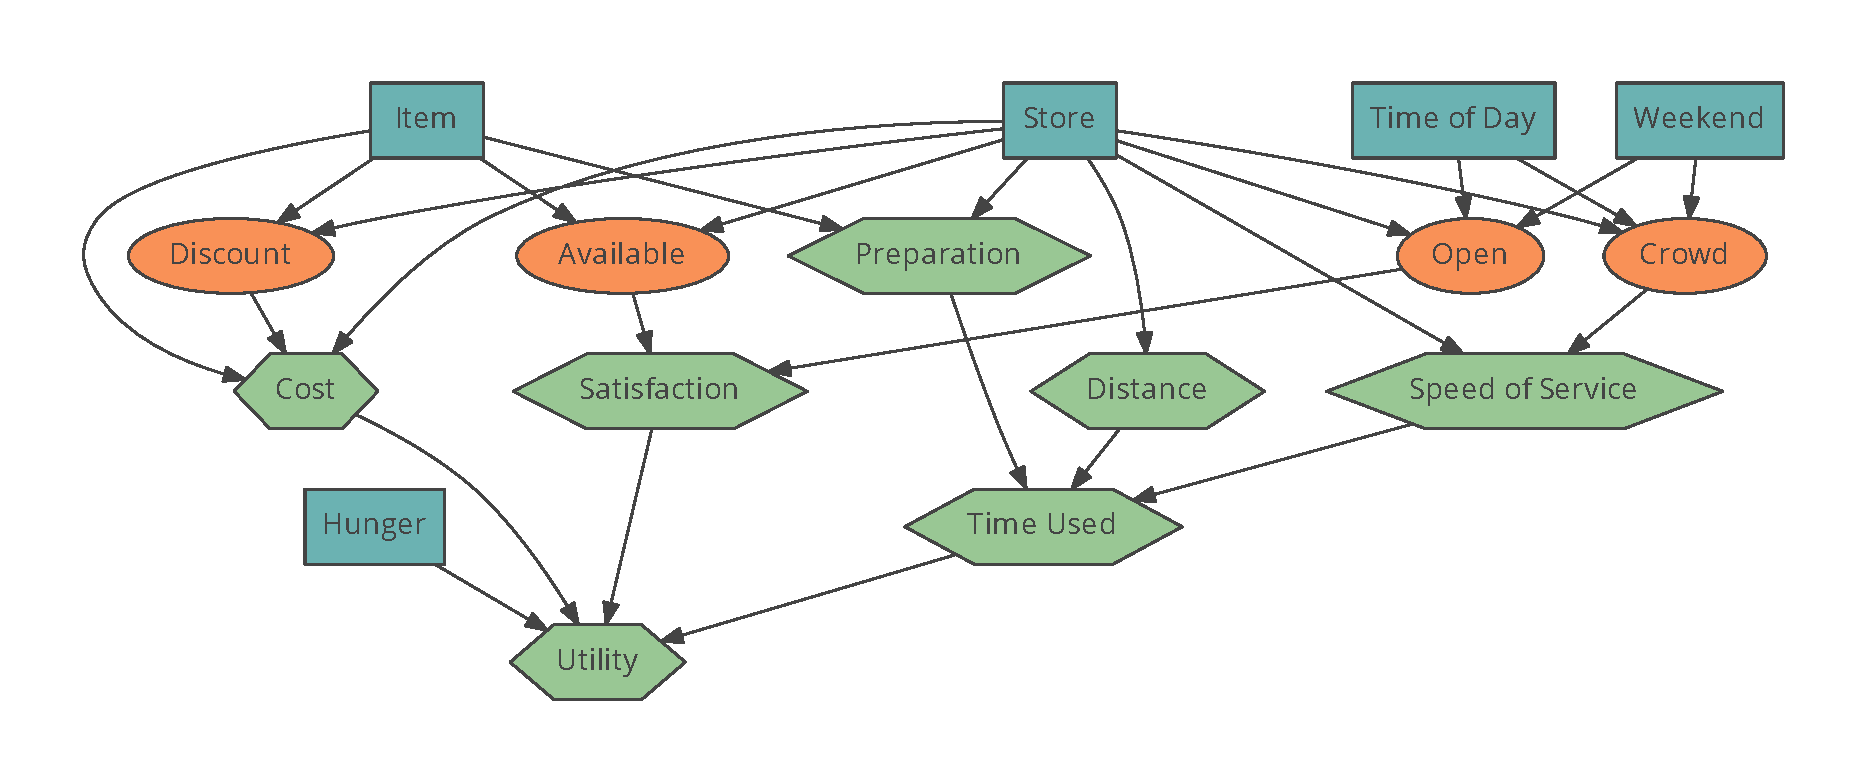
\includegraphics[scale=0.45]{model}
\caption{Model visualization showing \textit{decision nodes} (blue), \textit{chance nodes} (orange), and \textit{utility nodes} (green).}
\label{fig:model}
\end{figure}

\section{Model}

\subsection{Assumptions}

The following assumptions have been made in the modeling representation to reduce complexity:

\begin{enumerate}
\item The user only purchases one item at a time when visiting a store. An item in this context can be a set of related goods, e.g. ``Eggs \& Bacon''.
\item Discounts are modelled as being binary, with an item being 50\% cheaper if it is discounted. The probability of an item being discounted is a function of the store and the item, and an item can either be discounted or not.
\item To maintain some temporal resolution while keeping the model simple, only the hours 12:00 to 24:00 is modelled.
\item Item discount and item availability are both independent of whether it is a weekday or weekend, and the time of day.
\item Whether an item is available only depends on the item and on the store, it does not depend on the time or how crowded the store is.
\item The value of time and money are linear within the ranges used.
\end{enumerate}

The following conditional independencies are assumed:

\begin{enumerate}
\item \textit{Speed of Service} is assumed to be conditionally independent of \textit{Weekend} and \textit{Time of Day}, given the \textit{Crowdedness} of the store.
\item \textit{Open} and \textit{Crowd} are conditionally independent of each other given \textit{Weekend}, \textit{Time of Day} and \textit{Store}.
\item \textit{Open} and \textit{Available} are conditionally independent given 
\textit{Store}.
\end{enumerate}

\begin{table}
{\footnotesize
\centering
\begin{tabular}{cccc}
\toprule
Type & Known & Name           & Values \\
\midrule
Chance  & No  & Discount & Probability\\
Chance  & No  & Available & Probability\\
Chance  & No  & Open & Probability \\
Chance  & No  & Crowd & \textit{None}, \textit{Some}, \textit{Very} \\
Utility & Yes & Preparation & Duration in seconds \\
Utility & No  & Cost & Cost in NOK \\
Utility & No  & Satisfaction & Probability \\
Utility & Yes & Distance & Travel duration in seconds \\
Utility & No  & Speed of service & Time in seconds \\
Utility & No  & Time used & Time in seconds \\
\bottomrule
\end{tabular}
\caption{List of internal model variables. ``Known'' refers to whether the information is fully known at the time when the decision is made.}
\label{table:variables}
}
\end{table}

\subsection{Discount}

As discussed in the assumptions section, store discounts are modelled as a single probability per store-item pair, indicating the chance of an item being discounted. If an item is discounted, the price of the item will be 50\% of its nominal price.

The probability values listed in Table~\ref{table:discounts} are based on anecdotal evidence, both because our discount model is highly simplified, and due to the work required in tracking discounts at stores over long enough time to build correct averages. 

\begin{table}
\centering
\begin{tabular}{ccccc}
\toprule
& \textit{Bunnpris~Elgeseter} & \textit{Sesam~Samfundet} & \textit{Rema~1000~Elgeseter} & \textit{Shell~Elgeseter} \\
\midrule
\textit{Hamburger}     & 0.1  & 0.0 & 0.1  & 0.15 \\
\textit{Eggs \& Bacon} & 0.1  & 0.0 & 0.1  & 0.0 \\
\textit{Coca-Cola}     & 0.05 & 0.0 & 0.05 & 0.1 \\
\textit{Taco}          & 0.2  & 0.0 & 0.2  & 0.0 \\
\bottomrule
\end{tabular}
\caption{Probability of an item being discounted}
\label{table:discounts}
\end{table}

\subsection{Available}

Availability, see Table~\ref{table:available}, is defined as the probability of all components of an item being available for purchase at a given store at any time.

\begin{table}
\centering
\begin{tabular}{ccccc}
\toprule
& \textit{Bunnpris~Elgeseter} & \textit{Sesam~Samfundet} & \textit{Rema~1000~Elgeseter} & \textit{Shell~Elgeseter} \\
\midrule
\textit{Hamburger}     & 0.85  & 0.95 & 0.90  & 0.9 \\
\textit{Eggs \& Bacon} & 0.95  & 0.0 & 0.95  & 0.0 \\
\textit{Coca-Cola}     & 0.95  & 0.8 & 0.97 & 0.95 \\
\textit{Taco}          & 0.80  & 0.0 & 0.85  & 0.0 \\
\bottomrule
\end{tabular}
\caption{Probability of an item being available}
\label{table:available}
\end{table}

\subsection{Open}

In order to calculate the probability of a store being open or closed we took into account the usual store opening times together with an assigned uncertainty for whether the store would actually be open when it was scheduled to be open. Using Equations~\ref{eq:open1}-\ref{eq:open3}, a probability for the store being opened, given whether it is a weekday or weekend and the time period of the day, is calculated for each store. The first two formulas are weekday specific, but are identical for the weekend.

{\footnotesize

\begin{equation}
P(\mathit{Open} \vert \mathit{Store}, \mathit{Weekday},\mathit{TimePeriod}) = P(\mathit{Open} \vert \mathit{ScheduledOpen}) \cdot P(\mathit{ScheduledOpen} \vert \mathit{Store}, \mathit{Weekday},\mathit{TimePeriod})
\label{eq:open1}
\end{equation}

\begin{equation}
P(\mathit{ScheduledOpen} \vert \mathit{Store}, \mathit{Weekday},\mathit{TimePeriod}) = \frac{1}{n_{\mathit{weekdays}}} \cdot \sum_{d \in \mathit{Weekday}} P(\mathit{ScheduledOpen} \vert \mathit{Store}, d, \mathit{TimePeriod})
\label{eq:open2}
\end{equation}

\begin{equation}
P(\mathit{ScheduledOpen} \vert \mathit{Store}, \mathit{Day}, \mathit{TimePeriod}) = \frac{\mathit{HoursOpen}(\mathit{Store}, \mathit{TimePeriod})}{\mathit{Hours}(\mathit{TimePeriod})}
\label{eq:open3}
\end{equation}
}

\subsection{Crowd}

When visiting a store, how crowded the store is will affect the time it takes to shop there. ``Crowdedness'' is modelled as a function of both the store and point of time, and can either be ``none'', ``some'', or ``very''. Each of the three outcomes is assigned a probability between 0 and 1 for each point of time. The probabilities set in Table~\ref{table:crowd} are based on anecdotal evidence, and based on the observations that grocery stores are more busy during daytime; especially lunch and after work, and that all stores are more busy during weekends.

\begin{table}
{\footnotesize
\centering
\begin{tabular}{cccccc}
\toprule
& & \textit{Bunnpris~Elgeseter} & \textit{Sesam~Samfundet} & \textit{Rema~1000~Elgeseter} & \textit{Shell~Elgeseter} \\
\midrule
\multirow{4}{*}{Weekday} &
\textit{12-15} & 0.1, 0.6, 0.3 & 1.0, 0.0, 0.0 & 0.1, 0.6, 0.3 & 0.5, 0.3, 0.2 \\ &
\textit{15-18} & 0.1, 0.5, 0.4 & 0.8, 0.2, 0.0 & 0.1, 0.5, 0.4 & 0.5, 0.3, 0.2 \\ &
\textit{18-21} & 0.4, 0.4, 0.2 & 0.7, 0.2, 0.1 & 0.4, 0.4, 0.2 & 0.7, 0.2, 0.1 \\ &
\textit{21-24} & 0.8, 0.2, 0.0 & 0.1, 0.7, 0.2 & 0.8, 0.2, 0.0 & 0.8, 0.1, 0.1 \\
\midrule
\multirow{4}{*}{Weekend} &
\textit{12-15} & 0.1, 0.5, 0.4 & 1.0, 0.0, 0.0 & 0.1, 0.5, 0.4 & 0.5, 0.3, 0.2 \\ &
\textit{15-18} & 0.1, 0.5, 0.4 & 0.7, 0.2, 0.1 & 0.1, 0.5, 0.4 & 0.5, 0.3, 0.2 \\ &
\textit{18-21} & 0.3, 0.5, 0.2 & 0.6, 0.3, 0.1 & 0.3, 0.5, 0.2 & 0.5, 0.3, 0.2 \\ &
\textit{21-24} & 0.5, 0.4, 0.1 & 0.1, 0.6, 0.3 & 0.5, 0.4, 0.1 & 0.6, 0.2, 0.2 \\
\bottomrule
\end{tabular}
\caption{Probability of a store being crowded (\textit{None}, \textit{Some},
\textit{Very})}
\label{table:crowd}
}
\end{table}

\subsection{Preparation time}

For this task we assume that the preparation time for each meal is only dependent on the meal, and on where it was bought from. We assume also a that preparation time varies very little from time to time, and this variation has little to no effect on the decision we are modeling, and therefore choose to model it as a constant. Table~\ref{table:preparation} shows common preparation times found on the internet. When the food is prepared at the store, then preparation time represents how much time the store takes to prepare the food.

\begin{table}
\centering
\begin{tabular}{ccccc}
\toprule
& \textit{Bunnpris~Elgeseter} & \textit{Sesam~Samfundet} & \textit{Rema~1000~Elgeseter} & \textit{Shell~Elgeseter} \\
\midrule
\textit{Hamburger}     & 1800~\cite{hamburger_url}  & 300 & 1800~\cite{hamburger_url}  & 480 \\
\textit{Eggs \& Bacon} & 900~\cite{taco_url}  & 0 & 900~\cite{taco_url}  & 0 \\
\textit{Coca-Cola}     & 0 & 0 & 0 & 0 \\
\textit{Taco}          & 2400  & 0 & 2400  & 0 \\
\bottomrule
\end{tabular}
\caption{Preparation time in seconds.}
\label{table:preparation}
\end{table}

\subsection{Cost}

The cost of an item is modeled as static, meaning that the cost of items do not change in time and the only factor that affects the final price of an item is discounts.

The costs stated in Table~\ref{table:discounts} are based on information obtained on the internet, and from the stores themselves.

\begin{table}
\centering
\begin{tabular}{ccccc}
\toprule
& \textit{Bunnpris~Elgeseter} & \textit{Sesam~Samfundet} & \textit{Rema~1000~Elgeseter} & \textit{Shell~Elgeseter} \\
\midrule
\textit{Hamburger}     & 60  & 95 & 50  & 115 \\
\textit{Eggs \& Bacon} & 45  & 0.0 & 40  & 0.0 \\
\textit{Coca-Cola}     & 20 & 25 & 20 & 28 \\
\textit{Taco}          & 50  & 0.0 & 45  & 0.0 \\
\bottomrule
\end{tabular}
\caption{Non-discounted cost of items given the store.}
\label{table:cost}
\end{table}

\subsection{Satisfaction}

We define satisfaction, see Equation~\ref{eq:satisfaction}, as the probability of obtaining the desired item. This is determined by the probability of the item being available, and the probability of the store being open. Given that they are conditionally independent of each other given the store, the function used is:

\begin{equation}
\mathit{Satisfaction}(\mathit{Open}, \mathit{Available}) = \mathit{Open} \cdot \mathit{Available}
\label{eq:satisfaction}
\end{equation}

\subsection{Distance}

The distance for each store was found through measurements using the \textit{Google~Earth} tool. Measurements were made with a starting point at the intersection between the two authors; at latitude $63.418095^\circ$ and longitude $10.396682^\circ$. Each of the distances measured were then doubled to account for the travel in both directions.

The mean walking speed for young males is 1.5~$\frac{\text{meters}}{\text{second}}$\cite{carey2005establishing}. Using this as a conversion factor, each distance can be converted to a duration which can be unified with other metrics into a utility value.

The distances (both travel and return), (and corresponding durations), were found to be
\begin{enumerate*}
\item \textit{Bunnpris~Elgeseter} (400~meter; 267~seconds),
\item \textit{Sesam~Samfundet} (1000~meter; 667~seconds),
\item \textit{Rema~1000~Elgeseter} (760~meter; 507~seconds),
\item \textit{Shell~Elgeseter} (500~meter; 334~seconds).
\end{enumerate*}

\subsection{Speed of Service}

The speed of service, see Table~\ref{table:sos}, is defined as the amount of time used from entering a store to obtaining the item to be purchased. It is considered to be independent of the item being purchased, and depends only on the store and on how crowded it is.

\begin{table}
\centering
\begin{tabular}{ccccc}
\toprule
& \textit{Bunnpris~Elgeseter} & \textit{Sesam~Samfundet} & \textit{Rema~1000~Elgeseter} & \textit{Shell~Elgeseter} \\
\midrule
\textit{None} & 300  & 120  & 360  & 120 \\
\textit{Some} & 600  & 300  & 720  & 300 \\
\textit{Very} & 900  & 1200 & 1080 & 900 \\
\bottomrule
\end{tabular}
\caption{Speed of service in seconds given the store and level of crowdedness.}
\label{table:sos}
\end{table}

\subsection{Utility}

The utility function we use for this model, see Equation~\ref{eq:utility} is a function of time used, satisfaction, cost and hunger. These are the main properties that a person takes into account when choosing a store to buy from. Satisfaction affects the utility independently of the other factors, and it's importance is dependant on the hunger level. The effect of time depends on hunger, if hunger is large time must be less to maintain the same utility. The affect of cost also depends on hunger, if hunger is low then cost must be low to maintain the same utility. And finally if hunger is kept constant and time increases, then the cost must decrease to maintain the same utility.\\

\begin{equation}
\mathit{Satisfaction}^{\frac{1}{0.8 + \mathit{Hunger}}} \cdot \Bigg(\frac{1}{\big((1 - \mathit{Hunger}) \cdot \mathit{Cost}\big) + \big(\mathit{Hunger} \cdot \frac{\mathit{TimeUsed}*150}{3600}\big)}\Bigg)
\label{eq:utility}
\end{equation}

To tune the relation between time and money we used the \textit{Almanac Game}, where we each wrote down the 25\textsuperscript{th}, 50\textsuperscript{th}, and 75\textsuperscript{th} percentile for how much money, in \textit{Norwegian Kroner}, we each believe one hour of time is worth. The results were as follows, Per~Magnus had NOK 50, NOK 150 and NOK 400, and Alfredo had NOK 100, NOK 150, and NOK 200. We decided to use the two medians, NOK 150, for the final value. The \textit{TimeUsed} value is then scaled to a monetary value through multiplying with the ratio $\frac{150}{3600}\frac{\text{NOK}}{\text{second}}$.\\

Finally the effects of hunger are as follows: when hunger is \textit{None} an hour is worth NOK 37.5, when hunger is \textit{Some} an hour is worth NOK 150, and when hunger is \textit{Very} an hour is calculated at NOK 600.

\section{Evaluation}

The model was verified and evaluated by creating the gold standard shown in Table~\ref{table:evaluation}. The table was created by the authors after the inputs and outputs had been the define, and before the model was developed further. It was used to verify that the model gave results similar to the ones expected. Once the model was finished, the examples from the gold standard were evaluated using the model, giving the outputs shown in Table~\ref{table:evaluation}.

With minimal tuning the model managed to output decisions similar to the ones expected on Table~\ref{table:evaluation}. The single observed difference between the expected and the obtained results was the model's suggestion of going to \textit{Sesam Samfundet} given the parameters of Example~\#2. After discussing this scenario amongst the authors, we came to the conclusion that Per~Magnus would happily follow this suggestion, however Alfredo would most likely not.

Given that the model gave good results for the examples it was tested on, it should also give reasonable suggestions for other input combinations, aiding in the arduous task of human decision making.

\begin{table}
{\footnotesize
\centering
\begin{tabular}{cccccc}
\toprule
Type of food & Day & Time of day & Hunger & Expected Action & Model Recommendation \\
\midrule
\textit{Hamburger}     & \textit{Weekend} & \textit{21-24} & \textit{Very} & \textit{Sesam}    & \textit{Sesam} \\
\textit{Hamburger}     & \textit{Weekday} & \textit{15-18} & \textit{Some} & \textit{Rema1000} & \textit{Sesam} \\
\textit{Taco}          & \textit{Weekend} & \textit{12-15} & \textit{Very} & \textit{Bunnpris} & \textit{Bunnpris} \\
\textit{Eggs \& bacon} & \textit{Weekend} & \textit{12-15} & \textit{Some} & \textit{Bunnpris} & \textit{Bunnpris} \\
\textit{Coca-Cola}     & \textit{Weekend} & \textit{21-24} & \textit{Some} & \textit{Shell}    & \textit{Shell} \\
\bottomrule
\end{tabular}
\caption{Gold standard of input-output pairs}
\label{table:evaluation}
}
\end{table}

\bibliographystyle{plain}
\bibliography{references}

\end{document}
